\documentclass[12pt, a4paper, oneside, openright, titlepage]{book}
\usepackage[utf8]{inputenc}
\raggedbottom
\usepackage{import}


%%%%%%%%%%%%%%%%% Book Formatting Comments:

%%%%%%%%%%%%%%%%%%%%%%%%%%%%%%%%%%%%% for Part

%%%%%%%%%%%%%%%%%%%%%% for chapter

%%%%%%%%%%%%%%%%%%%% for section




%%%%%% PACKAGES %%%%%%%
\usepackage{hyperref}
\hypersetup{
    colorlinks,
    citecolor=black,
    filecolor=black,
    linkcolor=black,
    urlcolor=black
}
\usepackage{amsmath} % Math display options
\usepackage{amssymb} % Math symbols
%\usepackage{amsfonts} % Math fonts
%\usepackage{amsthm}
\usepackage{mathtools} % General math tools
\usepackage{array} % Allows you to write arrays
\usepackage{empheq} % For boxing equations
% \usepackage{mathabx}
% \usepackage{mathrsfs}
\usepackage{nameref}
\usepackage{wrapfig}

\usepackage{soul}
\usepackage[normalem]{ulem}

\usepackage{txfonts}
\usepackage{cancel}
\usepackage[toc, page]{appendix}
\usepackage{titletoc,tocloft}
\setlength{\cftchapindent}{1em}
\setlength{\cftsecindent}{2em}
\setlength{\cftsubsecindent}{3em}
%\setlength{\cftsubsubsecindent}{4em}
\usepackage{titlesec}

%\titleformat{\section}
%  {\normalfont\fontsize{25}{15}\bfseries}{\thesection}%{1em}{}
%\titleformat{\section}
%  {\normalfont\fontsize{20}{15}\bfseries}%{\thesubsection}{1em}{}
%\setcounter{secnumdepth}{1}  
  
  

%\newcommand\numberthis{\refstepcounter{equation}\tag{\theequation}} % For equation labelling
\usepackage[framemethod=tikz]{mdframed}

\usepackage{tikz} % For drawing commutative diagrams
\usetikzlibrary{cd}
\usetikzlibrary{calc}
\tikzset{every picture/.style={line width=0.75pt}} %set default line width to 0.75p

\usepackage{datetime}
\usepackage[margin=1.5in]{geometry}
\setlength{\parskip}{1em}
\usepackage{makeidx}         % allows index generation
\usepackage{graphicx}       % standard LaTeX graphics tool
\usepackage{multicol}        % used for the two-column index
\usepackage[bottom]{footmisc}% places footnotes at page bottom

\usepackage{newtxtext}       % 
\usepackage{newtxmath}       % selects Times Roman as basic font
\usepackage{float}
\usepackage{fancyhdr}
\setlength{\headheight}{15pt} 
\pagestyle{fancy}
\lhead[\leftmark]{}
\rhead[]{\leftmark}

%\usepackage{enumitem}

\usepackage{url}
\allowdisplaybreaks

%%%%%% ENVIRONMENTS %%%
\definecolor{purp}{rgb}{0.29, 0, 0.51}
\definecolor{bloo}{rgb}{0, 0.13, 0.80}



%%\newtheoremstyle{note}% hnamei
%{3pt}% hSpace above
%{3pt}% hSpace belowi
%{}% hBody fonti
%{}% hIndent amounti
%{\itshape}% hTheorem head fonti
%{:}% hPunctuation after theorem headi
%{.5em}% hSpace after theorem headi
%{}% hTheorem head spec (can be left empty, meaning ‘normal’)i





% %%%%%%%%%%%%% THEOREM DEFINITIONS

\spnewtheorem{axiom}{Axiom}[chapter]{\bfseries}{\itshape}


\spnewtheorem{construction}{Construction}[chapter]{\bfseries}{\itshape}

\spnewtheorem{props}{Properties}[chapter]{\bfseries}{\itshape}


\renewcommand{\qedsymbol}{$\blacksquare$}


\numberwithin{equation}{section}

\newenvironment{qest}{
    \begin{center}
        \em
    }
    {
    \end{center}
    }

%%%%%% MACROS %%%%%%%%%
%% New Commands
\newcommand{\ip}[1]{\langle#1\rangle} %%% Inner product
\newcommand{\abs}[1]{\lvert#1\rvert} %%% Modulus
\newcommand\diag{\operatorname{diag}} %%% diag matrix
\newcommand\tr{\mbox{tr}\.} %%% trace
\newcommand\C{\mathbb C} %%% Complex numbers
\newcommand\R{\mathbb R} %%% Real numbers
\newcommand\Z{\mathbb Z} %%% Integers
\newcommand\Q{\mathbb Q} %%% Rationals
\newcommand\N{\mathbb N} %%% Naturals
\newcommand\F{\mathbb F} %%% An arbitrary field
\newcommand\ste{\operatorname{St}} %%% Steinberg Representation
\newcommand\GL{\mathbf{GL}} %%% General Linear group
\newcommand\SL{\mathbf{SL}} %%% Special linear group
\newcommand\gl{\mathfrak{gl}} %%% General linear algebra
\newcommand\G{\mathbf{G}} %%% connected reductive group
\newcommand\g{\mathfrak{g}} %%% Lie algebra of G
\newcommand\Hbf{\mathbf{H}} %%% Theta fixed points of G
\newcommand\X{\mathbf{X}} %%% Symmetric space X
\newcommand{\catname}[1]{\normalfont\textbf{#1}}
\newcommand{\Set}{\catname{Set}} %%% Category set
\newcommand{\Grp}{\catname{Grp}} %%% Category group
\newcommand{\Rmod}{\catname{R-Mod}} %%% Category r-modules
\newcommand{\Mon}{\catname{Mon}} %%% Category monoid
\newcommand{\Ring}{\catname{Ring}} %%% Category ring
\newcommand{\Topp}{\catname{Top}} %%% Category Topological spaces
\newcommand{\Vect}{\catname{Vect}_{k}} %%% category vector spaces'
\newcommand\Hom{\mathbf{Hom}} %%% Arrows

\newcommand{\map}[2]{\begin{array}{c} #1 \\ #2 \end{array}}

\newcommand{\Emph}[1]{\textbf{\ul{\emph{#1}}}}




%% Math operators
\DeclareMathOperator{\ran}{Im} %%% image
\DeclareMathOperator{\aut}{Aut} %%% Automorphisms
\DeclareMathOperator{\spn}{span} %%% span
\DeclareMathOperator{\ann}{Ann} %%% annihilator
\DeclareMathOperator{\rank}{rank} %%% Rank
\DeclareMathOperator{\ch}{char} %%% characteristic
\DeclareMathOperator{\ev}{\bf{ev}} %%% evaluation
\DeclareMathOperator{\sgn}{sign} %%% sign
\DeclareMathOperator{\id}{Id} %%% identity
\DeclareMathOperator{\supp}{Supp} %%% support
\DeclareMathOperator{\inn}{Inn} %%% Inner aut
\DeclareMathOperator{\en}{End} %%% Endomorphisms
\DeclareMathOperator{\sym}{Sym} %%% Group of symmetries


%% Diagram Environments
\iffalse
\begin{center}
    \begin{tikzpicture}[baseline= (a).base]
        \node[scale=1] (a) at (0,0){
          \begin{tikzcd}
           
          \end{tikzcd}
        };
    \end{tikzpicture}
\end{center}
\fi




\newdateformat{monthdayyeardate}{%
    \monthname[\THEMONTH]~\THEDAY, \THEYEAR}
%%%%%%%%%%%%%%%%%%%%%%%

%%% Specific Macros %%%


%%%%%% BEGIN %%%%%%%%%%


\begin{document}

%%%%%% TITLE PAGE %%%%%%

\begin{titlepage}
    \centering
    \scshape
    \vspace*{\baselineskip}
    \rule{\textwidth}{1.6pt}\vspace*{-\baselineskip}\vspace*{2pt}
    \rule{\textwidth}{0.4pt}
    
    \vspace{0.75\baselineskip}
    
    {\LARGE Complex Analysis: A Complete Guide}
    
    \vspace{0.75\baselineskip}
    
    \rule{\textwidth}{0.4pt}\vspace*{-\baselineskip}\vspace{3.2pt}
    \rule{\textwidth}{1.6pt}
    
    \vspace{2\baselineskip}
    Complex Analysis \\
    \vspace*{3\baselineskip}
    \monthdayyeardate\today \\
    \vspace*{5.0\baselineskip}
    
    {\scshape\Large Elijah Thompson, \\ Physics and Math Honors\\}
    
    \vspace{1.0\baselineskip}
    \textit{Solo Pursuit of Learning}
    \vfill
    \enlargethispage{1in}
    \begin{figure}[b!]
    \makebox[\textwidth]{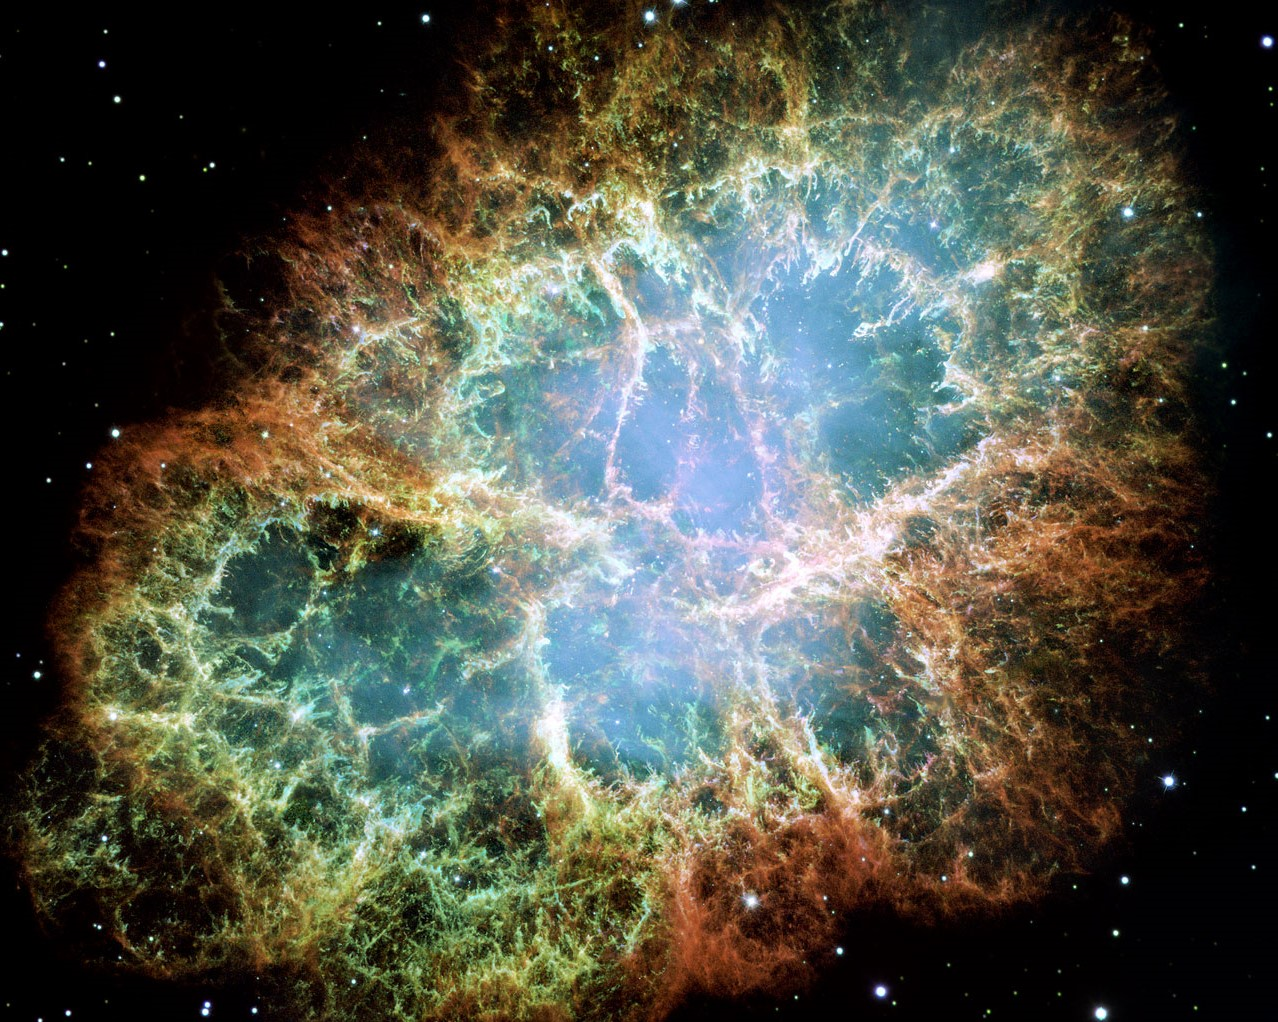
\includegraphics[width=\paperwidth, height =10cm]{../../Crab.jpg}}
    \end{figure}
\end{titlepage}

%%%%%%%%%%%%%%%%%%%%%%%
\tableofcontents


%%%%%%%%%%%%%%%%%%%%%%%%%%%%%%%%%%%%% Part 1.
\part{Part 1}

%%%%%%%%%%%%%%%%%%%%%% Chapter 1.1
\chapter{The Complex Plain and Basic Functions}




%%%%%%%%%%%%%%%%%%%% Section 1.1.1
\section{Complex Numbers}

The complex numbers, $\C$, consist of all formul sums $z = x+iy$, for $x,y \in \R$, where $i^2 = -1$ is the root of $x^2 + 1 = 0$. Then, for multiplication we proceed by $z\cdot w = (a+ib)(x+iy) = (ax-by)+i(xb+ay)$.

Gauss concieved of $\C$ as $\R^2$ with a binary operation $*$, where $(a,b)*(x,y) = (ax-by,xb+ay)$. Then, we observe that $(1,0)*(a,b) = (a,b)$, so $(1,0)$ acts as $1$. Moreover, $(0,1)*(0,1) = (-1,0) = -(1,0)$. 


The matrix model of $\C$ is $$\C = \left\{\begin{bmatrix} a & -b // b & a \end{bmatrix}: a,b \in \R\right\}$$

In terms of extension fields, we can consider $\C$ to be $\R[x]/(x^2+1)$. 

\begin{defn}
    If $z = x+iy$, with $x,y \in \R$, then we define $\mathscr{R}e(z) = x$ and $\mathscr{I}m(z) = y$.
\end{defn}


\begin{defn}
    If $z = x+iy$, we define the \Emph{conjugate} of $z$ to be $\overline{z} x-iy$.
\end{defn}

\begin{props}
    Let $z,w \in \C$. \begin{itemize}
        \item $\overline{z+w} = \overline{z}+\overline{w}$
        \item $\overline{zw} = \overline{z}\cdot \overline{w}$
        \item $\overline{\overline{z}} = z$
        \item $\overline{z} = 0$ if and only if $z = 0$
        \item $\mathscr{R}e(z) = \frac{z+\overline{z}}{2}$
        \item $\mathscr{I}m(z) = \frac{z-\overline{z}}{2i} = \frac{i(\overline{z}-z)}{2}$
    \end{itemize}
\end{props}

\begin{prop}
    If $z \neq 0$, then $z^{-1} = \frac{\overline{z}}{z\overline{z}}$.
\end{prop}


\begin{defn}
    Let $z \in \C$. Then the \Emph{modulus}, $|\cdot |$ of $z=a+ib$ (the norm), is the length of $z$ as a vector: \begin{equation*}
        |z| = \sqrt{a^2+b^2} = \sqrt{z\overline{z}}
    \end{equation*}
\end{defn}


\subsection{Geometry of the Complex Numbers}

The complex numbers, $\C = \{a+ib:a,b \in \R\}$, can be considered as a plane of points, or we can consider the complex numbers as vectors in the plane eminating from $0$. 
\begin{center}
	\begin{tikzpicture}[x=0.75pt,y=0.75pt,yscale=-1,xscale=1]
%uncomment if require: \path (0,398); %set diagram left start at 0, and has height of 398

%Straight Lines [id:da39464285181286485] 
\draw [color={rgb, 255:red, 255; green, 0; blue, 0 }  ,draw opacity=1 ]   (200,310) -- (287.66,212.27) ;
\draw [shift={(289,210.78)}, rotate = 491.89] [color={rgb, 255:red, 255; green, 0; blue, 0 }  ,draw opacity=1 ][line width=0.75]    (10.93,-3.29) .. controls (6.95,-1.4) and (3.31,-0.3) .. (0,0) .. controls (3.31,0.3) and (6.95,1.4) .. (10.93,3.29)   ;
%Straight Lines [id:da13724064512600265] 
\draw  [dash pattern={on 0.84pt off 2.51pt}]  (289,210.78) -- (289.67,309.44) ;
%Shape: Arc [id:dp896874676115538] 
\draw  [draw opacity=0][fill={rgb, 255:red, 74; green, 144; blue, 226 }  ,fill opacity=1 ][dash pattern={on 0.84pt off 2.51pt}] (211.58,297.56) .. controls (212.75,299.62) and (213.81,301.84) .. (214.75,304.19) .. controls (215.48,306.03) and (216.1,307.86) .. (216.61,309.67) -- (199.73,310.18) -- cycle ; \draw  [dash pattern={on 0.84pt off 2.51pt}] (211.58,297.56) .. controls (212.75,299.62) and (213.81,301.84) .. (214.75,304.19) .. controls (215.48,306.03) and (216.1,307.86) .. (216.61,309.67) ;
%Shape: Axis 2D [id:dp8729881414013165] 
\draw  (182.33,310.18) -- (356.33,310.18)(199.73,166.78) -- (199.73,326.11) (349.33,305.18) -- (356.33,310.18) -- (349.33,315.18) (194.73,173.78) -- (199.73,166.78) -- (204.73,173.78)  ;
%Straight Lines [id:da5981962432151724] 
\draw [color={rgb, 255:red, 74; green, 144; blue, 226 }  ,draw opacity=1 ]   (199.73,310.18) -- (130.17,214.18) ;
\draw [shift={(129,212.56)}, rotate = 414.07] [color={rgb, 255:red, 74; green, 144; blue, 226 }  ,draw opacity=1 ][line width=0.75]    (10.93,-3.29) .. controls (6.95,-1.4) and (3.31,-0.3) .. (0,0) .. controls (3.31,0.3) and (6.95,1.4) .. (10.93,3.29)   ;
%Shape: Arc [id:dp8546612577752639] 
\draw  [draw opacity=0][fill={rgb, 255:red, 243; green, 19; blue, 19 }  ,fill opacity=1 ][dash pattern={on 0.84pt off 2.51pt}] (194.73,303.29) .. controls (196.25,302.4) and (198.06,301.89) .. (200,301.89) .. controls (205.33,301.89) and (209.65,305.75) .. (209.67,310.53) -- (200,310.56) -- cycle ; \draw  [dash pattern={on 0.84pt off 2.51pt}] (194.73,303.29) .. controls (196.25,302.4) and (198.06,301.89) .. (200,301.89) .. controls (205.33,301.89) and (209.65,305.75) .. (209.67,310.53) ;

% Text Node
\draw (354,302.4) node [anchor=north west][inner sep=0.75pt]    {$\mathscr{R} e$};
% Text Node
\draw (184.5,151.07) node [anchor=north west][inner sep=0.75pt]    {$\mathscr{I} m$};
% Text Node
\draw (290,199.51) node [anchor=north west][inner sep=0.75pt]  [font=\scriptsize]  {$z=a+ib$};
% Text Node
\draw (220,312.18) node [anchor=north west][inner sep=0.75pt]  [font=\scriptsize]  {$a=|z|\cos \theta $};
% Text Node
\draw (292.67,254.84) node [anchor=north west][inner sep=0.75pt]  [font=\scriptsize]  {$ib=i|z|\sin \theta $};
% Text Node
\draw (218,294.51) node [anchor=north west][inner sep=0.75pt]  [font=\scriptsize]  {$\theta $};
% Text Node
\draw (202.67,286.62) node [anchor=north west][inner sep=0.75pt]  [font=\scriptsize]  {$\beta $};
% Text Node
\draw (100,200.29) node [anchor=north west][inner sep=0.75pt]  [font=\scriptsize]  {$w=x+iy$};

\draw   (122.72, 166.5) circle [x radius= 5, y radius= 5]   ;
\draw   (123.55, 165.96) circle [x radius= 5, y radius= 5]   ;
\draw   (288.47, 51.73) circle [x radius= 5, y radius= 5]   ;
\draw   (372.18, 109) circle [x radius= 5, y radius= 5]   ;
\draw   (537.1, 23.04) circle [x radius= 5, y radius= 5]   ;
\draw   (249.38, 297.62) circle [x radius= 5, y radius= 5]   ;
\draw   (376.5, 243.59) circle [x radius= 5, y radius= 5]   ;
\draw   (414.3, 248.15) circle [x radius= 5, y radius= 5]   ;
\end{tikzpicture}	
\end{center}


Noting this geometric picture, we can write $z = |z|\cos\theta+i|z|\sin\theta = |z|(\cos\theta + i\sin\theta)$. Suppose we had another complex number $w = |w|(\cos\beta+i\sin\beta)$. Then we observe that \begin{align*}
    zw &= |z||w|(\cos\theta+i\sin\theta)(\cos\beta+i\sin\beta) \\
    &= |zw|(\cos\theta\cos\beta -\sin\theta\sin\beta + i(\sin\theta\cos\beta+\cos\theta\sin\beta)) \\
    &= |zw|(\cos(\theta+\beta)+i\sin(\theta+\beta))
\end{align*}
so complex multiplication aligns with angle addition in the plane.


\begin{defn}
    Define \Emph{Euler's Formula} \begin{equation*}
        e^{i\theta} = \cos\theta+i\sin\theta
    \end{equation*}
\end{defn}

From our above work we have that \begin{equation*}
    zw = (|z|e^{i\theta})(|w|e^{i\beta}) = |zw|e^{i(\theta+\beta)}
\end{equation*}
so \begin{equation*}
    e^{i\theta}e^{i\beta} = e^{i(\theta+\beta)}
\end{equation*}
The conjugate of $e^{i\theta}$ is \begin{equation*}
    \overline{e^{i\theta}} = \overline{\cos\theta+i\sin\theta} = \cos\theta-i\sin\theta=\cos(-\theta)+i\sin(-\theta) = e^{-i\theta}
\end{equation*}


\begin{prop}
    $e^{i\theta} = e^{i\beta}$ if and only if $\theta = \beta + 2\pi k$ for some $k \in \Z$.
\end{prop}

Then we have that $e^{i\theta} = e^{-i\theta}$ if and only if $\theta = \pi k$ for some $k \in \Z$.

\begin{defn}
    Let $z \in \C$. The \Emph{argument} of $z = |z|e^{i\theta}$ is $\arg(z) = \{\theta+2\pi k:k \in \Z\}$, and the \Emph{principal argument} of $z$, $\text{Arg}(z) = \theta_0$, where $z = |z|e^{i\theta_0}$ and $\theta_0 \in (-\pi,\pi]$.
\end{defn}


\begin{eg}
    Consider $z = -42-42i$. Then $|z| = 42\sqrt{2}$, and $\text{Arg}(z) = -\frac{3\pi}{4}$, so $z = 42\sqrt{2}e^{-i\frac{3\pi}{4}}$, and $\arg(z) = -\frac{3\pi}{4} + 2\pi\Z$.
\end{eg}

\begin{props}
    For $z,w \in \C$, $\arg(zw) = \arg(z)+\arg(w)$, but $\text{Arg}(zw) \neq \text{Arg}(z)+\text{Arg}(w)$.
\end{props}

\begin{thm}[DeMoivre's Theorem] \label{thm:DeMoivre}
    For all $n \in \Z$, \begin{equation*}
        (e^{i\theta})^n = e^{in\theta}
    \end{equation*}
\end{thm}
\begin{proof}
    We proceed by induction on $n \in \N$. If $n=1$ then $(e^{i\theta})^1 = e^{i1\theta}$, so the base case holds. Now, suppose that the claim holds for some $n \geq 1$. It follows that \begin{align*}
        (e^{i\theta})^{n+1} &= (e^{i\theta})^1(e^{i\theta})^n \\ 
        &= e^{i\theta}e^{in\theta} \tag{by I.H} \\
        &= e^{i(\theta+n\theta)} \\
        &= e^{i(n+1)\theta}
    \end{align*}
    completing the proof.
\end{proof}



\begin{defn}
    Suppose that $n \in \N$, $w,z \in \C$ such that $z^n = w$, then $z$ is said to be an \Emph{$n$th root of $w$}. Moreover, the set of all $n$th roots is dentoed $w^{1/n} \neq \sqrt[n]{w}$.
\end{defn}

Let $z^n = w$, where $z = \rho e^{i\theta}$. Then it follows that \begin{align*}
    (\rho e^{i\theta})^n &= w \\
    \rho^ne^{in\theta} &= |w|e^{i\text{Arg}(w)} \tag{by \ref{thm:DeMoivre}}
\end{align*}
This gives the two equations $\rho^n = |w|$ and $e^{in\theta} = e^{i\text{Arg}(w)}$, so $\rho = \sqrt[n]{|w|}$, and \begin{align*}
    n\theta &= \text{Arg}(w)+2\pi k \\
    \theta &= \frac{\text{Arg}(w)}{n}+\frac{2\pi k}{n}
\end{align*}
This gives the following result: 
\begin{cor}
    $$w^{1/n} = \left\{\sqrt[n]{|w|}e^{i\frac{\text{Arg}(w)}{n}}e^{i\frac{2\pi k}{n}}: k \in \Z\right\}$$
\end{cor}
\begin{defn}
    If $w = 1$, we have that \begin{equation*}
        1^{1/n} = \left\{e^{i\frac{2\pi k}{n}}:k\in \Z\right\}
    \end{equation*}
    These are the \Emph{$n$th roots of unity}.
\end{defn}

Then we observe that for any $w \in \C$, $$w^{1/n} = \sqrt[n]{|w|}e^{i\frac{\text{Arg}(w)}{n}}1^{1/n}$$


\begin{eg}
    Consider the fourth roots of $81i$, so $(81i)^{1/4}$. Then we have that \begin{align*}
        (81i)^{1/4} &= \sqrt[4]{81}e^{i\frac{\pi}{8}}1^{1/4} \\
        &= 3e^{i\frac{\pi}{8}}\{1,i,-1,-i\}
    \end{align*}
\end{eg}

\begin{eg}
    Let $w = \exp\left(\frac{2\pi i}{6}\right)$. Then \begin{align*}
        1^{1/6} &= \{z \in \C:z^6 = 1\} = \{w,w^2,w^3,w^4,w^5,w^6 = 1\}
    \end{align*}
    Note $w = e^{i\pi/3} = \cos(\pi/3)+i\sin(\pi/3) = \frac{1+i\sqrt{3}}{2}$. Now, if we consider the polynomial $f(z) = z^6 - 1$, we now know six roots for this polynomial. Then we can factor \begin{equation*}
        f(z) = \prod_{i=1}^6(z-w^i)
    \end{equation*}
    In short, to solve $z^n = \rho$, we take the $n$th roots of $\rho$, $\rho^{1/n}$. 
\end{eg}



\begin{eg}
    Consider $z^2+bz+c = 0$. Then completing the square we obtain $z \in \left\{\frac{-b+ (b^2-4c)^{1/2}}{2}\right\}$, where \begin{equation*}
        \left(\frac{b^2-4c}{2}\right)^{1/2} = \left\{\begin{array}{ccc} \sqrt{\left|\frac{b^2-4c}{2}\right|} & -\sqrt{\left|\frac{b^2-4c}{2}\right|} & if\;b^2-4c \geq 0 \\ \sqrt{\left|\frac{b^2-4c}{2}\right|}i & -\sqrt{\left|\frac{b^2-4c}{2}\right|}i & if\; b^2-4c < 0 \end{array}\right\}
    \end{equation*}
\end{eg}


%%%%%%%%%%%%%%%%%%%% Section 1.1.2
\section{Local Inverses and Branch-cut}

\begin{defn}    
    Let $z,w \in \C$, then the line segment from $z$ to $w$ is \begin{equation*}
        [z,w] = \{z+t(w-z):0\leq t \leq 1\}
    \end{equation*}
    where we also allow $z$ or $w$ to be plus or minus infinity.
\end{defn}

\begin{defn}
    The \Emph{negative slit plane}, $\C^-$, is defined by $\C^- = \C\backslash(-\infty,0]$, and the \Emph{positive slit plane}, $\C^+$, is defined by $\C^+ = \C\backslash[0,\infty)$. In general, we define \begin{equation*}
        C^{\alpha} = \C\backslash[0,e^{i\alpha}\infty)
    \end{equation*}
    to denote the exclusion of the ray along the $\alpha$th angle from the positive real axis.
\end{defn}

\begin{qst}
    What is a function?
\end{qst}

\begin{defn}
    If $f:S\rightarrow \C$ is a function, and $U \subseteq S$, then $f\vert_U:U\rightarrow \C$ is defined by $f\vert_U(z) = f(z)$ for all $z \in U$.
\end{defn}

We may have the case that $f$ is not injective (so it cannot be inverted). But, for a smart choice of $U$, we may have that $f\vert_U$ is one-to-one, and hence invertible. Such a restriction is known as a \Emph{local inverse} for $f$.

Rigourously, a \Emph{branch cut} is a curve in the complex plane such that it is possible to define a single analytic branch (sheets of a multivalued function) of a multivalued function on the plane minus that curve. That is, a branch is a way of making the multivalued function single valued, and in the context of determining inverses a branch is a choice of inverse.

\begin{eg}
    For $f(z) = z^n$, then for $U = \left\{z \in \C: -\frac{\pi}{n}<\text{Arg}(z) < \frac{\pi}{n}\right\}$, $f\vert_{U}$ is invertible, and $f\vert_{U}^{-1}$ is called the \Emph{principal branch}. $f\vert_U^{-1}$ is a choice of the $n$th root of $w \in \C^-$. 
\end{eg}


\begin{defn}
    The \Emph{$\alpha$-argument} for $\alpha \in \R$ is denoted $\text{Arg}_{\alpha}:\C^{\times}\rightarrow (\alpha,\alpha+2\pi)$. In particular, for each $z \in \C^{\times}$ we define $\text{Arg}_{\alpha} \in \arg(z)$ such that $z \in (\alpha,\alpha+2\pi)$
\end{defn}

We can give branch cuts for the $n$th root function which delete the ray at standard angle $\alpha$. These correspond to local inverse functions $f(z) = z^n$ restricted to $\{z \in \C^{\times}:\arg(z) = (\alpha/n,(\alpha+2\pi)/2)+2\pi\Z\}$.


\subsection{Square-Root Function}

If we have $z^2 = w$, this is equivalent to $(|z|e^{i\theta})^2 = |w|e^{i\beta}$, so $|z|^2=|w|$ and $e^{i2\theta} = e^{i\beta}$. Then $|z| = \sqrt{|w|}$, and $\theta = \frac{\beta}{2} + \pi k$ for $k \in \Z$. Then our solutions are \begin{equation*}
    z = \sqrt{|w|}e^{i(\beta/2+\pi k)} = \sqrt{|w|}e^{i\beta/2}e^{i\pi k} = \sqrt{|w|}e^{i\beta/2}\cos(\pi k)
\end{equation*}
Thus, in general \begin{equation*}
    z = \sqrt{|w|}e^{i\text{Arg}(w)/2}(-1)^k = \pm \sqrt{|w|}e^{i\text{Arg}(w)/2}
\end{equation*}
and \begin{equation*}
    w^{1/2} = \{\sqrt{|w|}e^{i\text{Arg}(w)/2}, -\sqrt{|w|}e^{i\text{Arg}(w)/2}\}
\end{equation*}
In general we have \begin{equation*}
    w^{1/n} = \{\sqrt[n]{w},\zeta\sqrt[n]{w},...,\zeta^{n-1}\sqrt[n]{w}\}
\end{equation*}
where $\sqrt[n]{w} = \sqrt[n]{|w|}\exp\left(\frac{i\text{Arg}(w)}{n}\right)$ is the principal root, and $\zeta = e^{\frac{2\pi i}{n}}$ is an $n$th root of unity. The principal root is the local inverse for the principal branch $U = 
\{z:-\pi/n < \text{Arg}(z) < \pi/n\}$. 


%%%%%%%%%%%%%%%%%%%% Section 1.1.3
\section{Complex Exponential}

\begin{defn}
    We define the complex exponential for $z \in \C$ to be \begin{equation*}
        e^z = e^{\mathscr{R}e(z)}e^{i\mathscr{I}m(z)} = e^{\mathscr{R}e(z)}(\cos(\mathscr{I}m(z))+i\sin(\mathscr{I}m(z)))
    \end{equation*}
\end{defn}

\begin{props}
    Let $z = x+iy, w = a+ib \in \C$. \begin{itemize}
        \item $e^ze^w = e^{z+w}$
        \item $|e^{x+iy}| = |e^x||e^{iy}| = e^x$, which is never zero so the complex exponential is never zero. that is,
        \item $e^z \neq 0$ for all $z \in \C$.
        \item $\arg(e^z) = \arg(e^xe^{iy}) = y+2\pi\Z$.
    \end{itemize}
\end{props}


\subsection{Failure to Inject}

If $e^{z_1} = e^{z_2}$, then $e^{x_1}e^{iy_1} = e^{x_2}e^{iy_2}$, so $x_1 = x_2$ and $y_1 \in y_2 + 2\pi\Z$. Thus, $e^z$ has a $2\pi i$-periodicity; $e^z = e^{z+2\pi ik}$ for $k \in \Z$. To make the complex exponential, we must restrict the domain to some horizontal strip of height at most $2\pi$ (with endpoints not included). In particular, if we take $U = \{x+iy: -\pi < y < \pi\}$ we obtain the branch $\C^-$, and branch cut $(-\infty,0]$. Then, suppose we write $e^z = w = |w|e^{i\text{Arg}(w)}$. Then a solution is $e^x = |w|$, and $y = \text{Arg}(w)$. We can then define \begin{equation*}
    \text{Log}(w) = \ln|w| +i\text{Arg}(w) = z = x+iy
\end{equation*}
for $w \in \C^-$, which is the branch cut to the multivalued log \begin{equation*}
    \log(z) = \ln|z|+i\arg(z)
\end{equation*}
taking the restriction $U$ in the range.



%%%%%%%%%%%%%%%%%%%% Section 1.1.4
\section{Sine, Cosine, Cosh, Sinh}

Recall $e^{i\theta} = \cos\theta +i\sin\theta$ and $e^{-i\theta} = \cos\theta-i\sin\theta$. Then we have that \begin{equation*}
    e^{i\theta}+e^{-i\theta}=2\cos\theta
\end{equation*}
and \begin{equation*}
    e^{i\theta}-e^{-i\theta} = 2i\sin\theta
\end{equation*}
Thus, we can obtain formulas for $\sin$ and $\cos$, $\theta \in \C$: \begin{equation*}
    \cos\theta = \frac{e^{i\theta}+e^{-i\theta}}{2}
\end{equation*}
and \begin{equation*}
    \sin\theta = \frac{e^{i\theta}-e^{-i\theta}}{2i}
\end{equation*}
Then we define:

\begin{defn}
    We define the complex sine and cosine, $z \in \C$, by \begin{equation}
        \boxed{\cos z = \frac{e^{iz}+e^{-iz}}{2}}
    \end{equation}
    and \begin{equation}
        \boxed{\sin z = \frac{e^{iz}-e^{-iz}}{2i}}
    \end{equation}
\end{defn}

Observe that \begin{equation*}
    e^x = \underbrace{\frac{1}{2}(e^x+e^{-x})}_{\cosh(x)} + \underbrace{\frac{1}{2}(e^x-e^{-x})}_{\sinh(x)}
\end{equation*}
\begin{defn}
    We define the complex hyperbolic sine and hyperbolic cosine, $z \in \C$, by \begin{equation}
        \boxed{\cosh z = \frac{e^{z}+e^{-z}}{2}}
    \end{equation}
    and \begin{equation}
        \boxed{\sinh z = \frac{e^{z}-e^{-z}}{2}}
    \end{equation}
\end{defn}

Then we have the identities \begin{equation*}
    \cosh z = \cos(iz), \sinh z = -i\sin(iz)
\end{equation*}
and \begin{equation*}
    \cos(z) = \cosh(iz), \sin z = -i\sinh(iz)
\end{equation*}

\subsection{Complex Cosine is Not Bounded}

Observe \begin{equation*}
    \cos(z) = \cos(x+iy) = \frac{e^{ix-y}+e^{-ix+y}}{2} = \frac{e^{ix}e^{-y}+e^{-ix}e^y}{2}
\end{equation*}
Now, using angle formulas we have \begin{align*}
    \cos(z) &= \cos(x+iy) \\
    &= \cos(x)\cos(iy)-\sin(x)\sin(iy) \\
    &= \cos(x)\cosh(y)-i\sin(x)\sinh(y)
\end{align*}
so \begin{equation*}
    |\cos z|^2 = \cos^2x\cosh^2y+\sin^2x\sinh^2y = \cos^2x+\sinh^2y
\end{equation*}
so as $\cosh$ and $\sinh$ are unbounded, so is complex $\cos$. 

\begin{claim}
    \begin{align*}
        \cos(z+w) &= \cos(z)\cos(w)-\sin(z)\sin(w) \\
        \sin(z+w) &= \sin(z)\cos(w)+\sin(w)\cos(z) 
    \end{align*}
    and \begin{align*}
        \cosh(z+w) &= \sinh z\sinh w + \cosh z\cosh w \\
        \sinh(z+w) &= \sinh z\cosh w + \cosh z\sinh w
    \end{align*}
\end{claim}


\begin{claim}
    $\cos^2z+\sin^2z = 1$
\end{claim}
\begin{proof}
    First, observe \begin{equation*}
        \cos^2z = \left[\frac{1}{2}(e^{iz}+e^{-iz})\right]^2 = \frac{1}{4}(e^{2iz}+2+e^{-2iz})
    \end{equation*}
    and \begin{equation*}
        \sin^2z = \left[\frac{1}{2i}(e^{iz}-e^{-iz})\right]^2 = \frac{-1}{4}(e^{2iz}-2+e^{-2iz})
    \end{equation*}
    Hence, indeed, $\cos^2z + \sin^2z = 1$.
\end{proof}


%%%%%%%%%%%%%%%%%%%% Section 1.1.5
\section{Power Functions}

\begin{defn}
    Let $\alpha \in \C$ be arbitrary. For $z \in \C^{\times}$ we define the power function $z^{\alpha}$ to be the multivalued function \begin{equation*}
        z^{\alpha} = e^{\alpha\log z}
    \end{equation*}
    Thus, the values of $z^{\alpha}$ are given by \begin{align*}
        z^{\alpha} &= e^{\alpha(\log|z| +i\arg(z))} \\
        &= e^{\alpha\text{Log}(z)}e^{2\pi i\alpha m}, m = 0, \pm 1,\pm 2,...
    \end{align*}
\end{defn}

Consequently, the various values of $z^{\alpha}$ are obtained by multiplying the principal value $e^{\alpha\text{Log}|z|}$ by the integer power of $e^{2\pi i\alpha}$. Consequently, if $\alpha$ is itself an integer $e^{2\pi i\alpha} = 1$, and the power function is single valued and equal to the principal value, $e^{\alpha\text{Log}|z|}$. If $\alpha = 1/n$, for $n \in \N$, then the factor is precisely the $n$th roots of unity, and $z^{1/n}$ are the $n$th roots of unity of $z$.

It is important to note that the usual algebraic rules do not apply to power functions when they are multivalued. 

To haze the power function move continuously with $z$ we make the branch cut $[0,\infty)$. Then we define a continuous branch on $\C^+$ to be \begin{equation*}
    w = r^{\alpha}e^{i\alpha \theta},\; \text{ for }\;z = re^{i\theta}, 0<\theta < 2\pi
\end{equation*}
At the top edge of the slit, $\theta = 0$, we have the usual power function $r^{\alpha} = e^{\alpha\text{Log}r}$. At the bottom of the slit, $\theta = 2\pi$, we have the function $r^{\alpha}e^{2\pi i\alpha}$. For a fixed $r$, as $\theta$ ranges the values of $w= r^{\alpha}e^{i\theta\alpha}$ move continuously. Thus, the values of this branch of $z^{\alpha}$ on the bottom edge are $e^{2\pi i\alpha}$ times the values at the top edge. This multiple, $e^{2\pi i\alpha}$, is called the \Emph{phase factor} of $z^{\alpha}$ at $z = 0$. 

For any other choice of branch, $w=r^{\alpha}e^{i\alpha(\theta+2\pi m)}$, the same phase factor is observed. 

\begin{lem}[Phase Change Lemma]\label{lem:phasechange}
    Let $g(z)$ be a single-valued function that is defined and continuous near $z_0$. For any continuously varying branch of $(z-z_0)^{\alpha}$ the function $f(z) = (z-z_0)^{\alpha}g(z)$ is multiplied by the phase factor $e^{2\pi i \alpha}$ when $z$ traverses acomplete circle about $z_0$ in the positive direction.
\end{lem}




%%%%%%%%%%%%%%%%%%%%%% Chapter 1.2
\chapter{Analytic Functions}



%%%%%%%%%%%%%%%%%%%%%% Chapter 1.3
\chapter{Line Integrals and Harmonic Functions}



%%%%%%%%%%%%%%%%%%%%%% Chapter 1.4
\chapter{Complex Integration and Analyticity}



%%%%%%%%%%%%%%%%%%%%%% Chapter 1.5
\chapter{Power Series}




%%%%%%%%%%%%%%%%%%%%%% Chapter 1.6
\chapter{Laurent Series and Isolated Singularities}



%%%%%%%%%%%%%%%%%%%%%% Chapter 1.7
\chapter{The Residue Calculus}



%%%%%%%%%%%%%%%%%%%%%%%%%%%%%%%%%%%%% Part 2.
\part{Part 2}

%%%%%%%%%%%%%%%%%%%%%% Chapter 2.1
\chapter{The Logarithmic Integral}




%%%%%%%%%%%%%%%%%%%%%% Chapter 2.2
\chapter{Conformal Mapping}





%%%%%%%%%%%%%%%%%%%%%%%%%%%%%%%%%%%%% Part 3.
\part{Part 3}

%%%%%%%%%%%%%%%%%%%%%% Chapter 3.1
\chapter{Approximation Theorems}




%%%%%%%%%%%%%%%%%%%%%% Chapter 3.2
\chapter{Special Functions}








%%%%%%%%%%%%%%%%%%%%%% - Appendices
\begin{appendices}


\end{appendices}


\end{document}


%%%%%% END %%%%%%%%%%%%%
